\chapter{MATHEMATICAL APPENDICES}
\section{Hermite polynomials}\label{Hermite polynomials}
The equation
\begin{equation}\label{a.1}
y''-2xy'+2ny=0
\end{equation}
belongs to a class which can be solved by what is called \textit{Laplace’s method}.\footnote{See, for instance, E. Goursat, \textit{Cours d’Analyse Mathematique}, Vol. II, Gauthier-Villars, Paris; V. I. Smirnov, \textit{Course of Higher Mathematics}, Vol. III, Part 2, Pergamon, Oxford, 1964.
}

This method is applicable to any linear equation of the form
\[ \sum_{m=0}^n(a_m+b_mx)\frac{\d^m y}{{\d x}^m}=0, \]
whose coefficients are of degree in $ x $ not higher than the first, and consists in the following procedure. We form the polynomials
\[ P(t)=\sum_{m=0}^na_mt^m,\quad Q(t)=\sum_{m=0}^nb_mt^m \]
and from them the function
\[ Z(t)=\frac{1}{Q}\exp\int\frac{P}{Q}\d t, \]
which is determined to within a constant factor. Then the solution of the equation under consideration can be expressed as a complex integral:
\[ y=\int_CZ(t)\e^{xt}\d t, \]
where the path of integration $ C $ is taken so that the integral is finite and non-zero, and the function
\[ V=\e^{xt}QZ \]
returns to its original value when $ t $ describes the contour $ C $ (which may be either closed or open).

In the case of equation \eqref{a.1} we have
\[ P=t^2+2n;\quad Q=-2t,\quad Z=\frac{1}{2t^{n+1}}\e^{-t^2/4},\quad V=\frac{1}{t^n}\e^{xt-t^2/4} ,\]
so that its solution is
\begin{equation}\label{a.2}
y=\int\exp\left(xt-\frac{t^2}{4} \right)\frac{\d t}{t^{n+1}}.
\end{equation}



For physical applications we need only consider values $ n > -1/2 $. For these values the contour of integration can be taken as $ C_1 $ or $ C_2 $ (Fig. \ref{Fig.52}); these satisfy the required conditions\footnote{These paths will not serve for negative integral $ n $, since the integral \eqref{a.2} along them then vanishes identically.
}, since the function $ V $ vanishes at their ends ($ t = +\infty $ or $ t = -\infty $).



Let us find the values of the parameter $ n $ for which equation \eqref{a.1} has solutions finite for all finite $ x $, which tend to infinity, as $ x \to\pm\infty $, not more rapidly than every finite power of $ x $. First, we consider non-integral values of $ n $. The integrals \eqref{a.2} along $ C_1 $ and $ C_2 $ then give two independent solutions of equation \eqref{a.1}. We transform the integral along $ C_1 $ by introducing the variable u such that $ t = 2(x - u) $. Omitting a constant factor, we find
\begin{equation}\label{a.3}
y=\e^{x^2}\int_{C_1'}\frac{\e^{-u^2}}{(u-x)^{n+1}}\d u,
\end{equation}
where the integration is taken over the contour $ C_1' $ in the complex plane of $ u $, as shown in Fig. \ref{Fig.53}.
\begin{figure}[H]
\parbox[]{.5\textwidth}{\begin{tikzpicture}
	\draw[-] (-2,1)--(2,1);
	\draw[-] (0,0.25)--(0,1.75);
	\draw[thick] (2, 1.25) [-{Stealth[length=10pt, angle'=30]}]-- (1.25, 1.25);
	\draw[thick] (1.35, 1.25) -- (0.25, 1.25) 
	arc[radius = 0.35355cm, start angle = 45, delta angle = 270]
	-- (0.25, 0.75) -- (1.35, 0.75)
	(1.25, 0.75) [{Stealth[length=10pt, angle'=30, reversed]}-]-- (2, 0.75);
	%\node[font=\large,above] at (0, 0) {$E_i$};
	\node[font=\large,above] at (1.25, 1.25) {$C_2$};
	%\fill (0, 0) circle(1.5pt);
	\draw[-] (-2,-1)--(2,-1);
	\draw[-] (0,-0.25)--(0,-1.75);
	\draw[thick] (-2, -1.25) [-{Stealth[length=10pt, angle'=30]}]-- (-1.25, -1.25);
	\draw[thick] (-1.35, -1.25) -- (-0.25, -1.25) 
	arc[radius = 0.35355cm, start angle = 225, delta angle = 270]
	-- (-0.25, -0.75) -- (-1.35, -0.75)
	(-1.25, -0.75) [{Stealth[length=10pt, angle'=30, reversed]}-]-- (-2, -0.75);
	\node[font=\large,above] at (-1.25, -0.75) {$C_1$};
	\node [font=\large] at (2,0) {$t$};
	\draw (2,0) circle (1.5ex);
	\end{tikzpicture}\caption{FIG. 52}\label{Fig.52}}
\parbox[]{.5\textwidth}{\begin{tikzpicture}
	\draw[-] (-2,1)--(2,1);
	\draw[-] (0,0.25)--(0,1.75);
	\draw[thick] (-2, 0.75) [-{Stealth[length=10pt, angle'=30]}]-- (-1.25, 0.75);
	\draw[thick] (-1.35, 0.75) -- (0.5, 0.75) 
	arc[radius = 0.35355cm, start angle = 225, delta angle = 270]
	-- (0.5, 1.25) -- (-1.35, 1.25)
	(-1.25,1.25) [{Stealth[length=10pt, angle'=30, reversed]}-]-- (-2, 1.25);
	\fill (0.75, 1) circle(2.5pt);
	%\node[font=\large,above] at (0, 0) {$E_i$};
	\node[font=\large,above] at (1.25, 1.25) {$x$};
	\node[font=\large,above] at (-1, 1.25) {$C_2'$};
	%\fill (0, 0) circle(1.5pt);
	\draw[-] (-2,-1)--(2,-1);
	\draw[-] (0,-0.25)--(0,-1.75);
	\draw[thick] (2, -0.75) [-{Stealth[length=10pt, angle'=30]}]-- (1.5, -0.75);
	\draw[thick] (1.75, -0.75) -- (1, -0.75) 
	arc[radius = 0.35355cm, start angle = 45, delta angle = 270]
	-- (1, -1.25) -- (1.75, -1.25)
	(1.5, -1.25) [{Stealth[length=10pt, angle'=30, reversed]}-]-- (2, -1.25);
	\node[font=\large,below] at (0.25, -1) {$x$};
	\node[font=\large,below] at (1.5, -1.25) {$C_1'$};
	\fill (0.75, -1) circle(2.5pt);
	\node [font=\large] at (2,0) {$u$};
	\draw (2,0) circle (1.5ex);
	\end{tikzpicture}\caption{FIG. 53}\label{Fig.53}}
\end{figure}







As $ x \to +\infty $, the whole path of integration $ C_1' $ moves to infinity, and the integral in \eqref{a.3} tends to zero as $ \e^{-x^2} $. As $ x \to-\infty $, however, the path of integration extends along the whole of the real axis, and the integral in \eqref{a.3} does not tend exponentially to zero, so that the function $ y (x) $ becomes infinite essentially as $ \e^{x^2} $ Similarly, it is easy to see that the integral \eqref{a.2} along the contour $ C_2 $ diverges exponentially as $ x \to+\infty $.

For positive integral $ n $ (including zero), on the other hand, the integrals along the straight parts of the path of integration cancel, and the two integrals \eqref{a.3}, along $ C_1' $ and $ C_2' $, reduce to an integral along a closed path round the point $ u = x $. Thus we have the solution
\[ y(x)=\e^{x^2}\oint\frac{\e^{-u^2}}{(u-x)^{n+1}}\d u, \]
which satisfies the conditions stated. According to Cauchy’s well-known formula for the derivatives of an analytic function,
\[ f^{(n)}(x)=\frac{n!}{2\pi\i}\oint\frac{f(t)}{(t-x)^{n+1}}\d t, \]
$ y (x) $ is, apart from a constant factor, an \textit{Hermite polynomial}:
\begin{equation}\label{a.4}
H_n(x)=(-1)^n\e^{x^2}\frac{\d^n}{{\d x}^n}\e^{-x^2}.
\end{equation}



The polynomial $ H_n $, expanded in decreasing powers of $ x $, has the open form
\begin{equation}\label{a.5}
H_n(x)=(2x)^n-\frac{n(n-1)}{1}(2x)^{n-2}+\frac{n(n-1)(n-2)(n-3)}{1\cdot2}(2x)^{n-4}-\dots
\end{equation}
It contains only powers of $ x $ which are of the same parity as $ n $. We may write out here the first few Hermite polynomials:
\begin{equation}\label{a.6}
H_0=1, H_1=2x, H_2=4x^2-2, H_3=8x^3-12x, H_4=16x^4-48x^2+12.
\end{equation}



To calculate the normalization integral, we replace $ \e^{-x} H_n $ by its expression in \eqref{a.4} and integrate $ n $ times by parts:
\[ \int_{-\infty}^{+\infty}\e^{-x^2}H_n^2(x)\d x=\int_{-\infty}^{+\infty}(-1)^nH_n(x)\frac{\d^n}{{\d x}^n}\e^{-x^2}\d x=\int_{-\infty}^{\infty}\e^{-x^2}\frac{\d^nH_n}{\d x^n}\d x. \]
But $\d^nH_n/{\d x}^n $ is a constant, $ 2^nn! $. Thus
\begin{equation}\label{a.7}
\int_{-\infty}^{+\infty}\e^{-x^2}H_n^2(x)\d x=2^nn!\sqrt{\pi}.
\end{equation}

\section{The Airy function}\label{The Airy function}
The equation
\begin{equation}\label{b.1}
y''-xy=0
\end{equation}
is of Laplace’s type (see \S\ref{Hermite polynomials}). Following the general method, we form the functions
\[ P=t^2,\quad Q=-1,\quad Z=-\exp(-t^3/3),\quad V=\exp(xt-t^3/3), \]
so that the solution can be represented in the form
\begin{equation}\label{b.2}
y(x)=\mathrm{const}\cdot\int_C\exp(xt-t^3/3)\d t,
\end{equation}
The path of integration $ C $ must be chosen so that the function $ V $ vanishes at both ends of it. These ends must therefore go to infinity in the regions of
\begin{wrapfigure}[]{l}[0cm]{0cm}
	\begin{tikzpicture}[scale=1.5]
	\draw[-] (-2,0)--(2,0);
	\draw[-] (0,-2)--(0,2);
	\draw[ domain =-1.73205:1.5,smooth] plot(\x,{0.57735*\x});
	\draw[ domain =-1.73205:1.5,smooth] plot(\x,{-0.57735*\x});
	\fill[pattern=north west lines] (-1.73205,-1) -- (0,0) -- (0,-2) --(210:2) arc (210:270:2)-- cycle;
	\draw (0,-0.5)[-{Stealth[length=3pt, angle'=60]}]--(270:0.5) arc(270:330:0.5);
	\draw (0.433,-0.25)[-{Stealth[length=3pt, angle'=60]}]--(330:0.5) arc(330:270:0.5);
	\node[font=\small,right] at (0, -0.75) {$\frac{\pi}{3}$};
	\draw (0,0.5)[-{Stealth[length=3pt, angle'=60]}]--(90:0.5) arc(90:30:0.5);
	\draw (0.433,0.25)[-{Stealth[length=3pt, angle'=60]}]--(30:0.5) arc(30:90:0.5);
	\node[font=\small,right] at (0, 0.75) {$\frac{\pi}{3}$};
	\node[font=\small,below] at (-0.5,-2) {$ C $};
	\draw[thick] (-0.5,-2)[-{Stealth[length=5pt, angle'=30]}]--(0.5,-1);
	\draw[thick] (0.25,-1.25)--(1.5,0);
	\draw[thick] (1.5,0)[-{Stealth[length=5pt, angle'=30]}]--(0.75,0.75);
	\draw[thick] (1,0.5)--(-0.4,1.9);
	\draw (1,0)[-{Stealth[length=3pt, angle'=60]}]--(1,0)arc[radius = 0.5cm, start angle = 180, delta angle = -45];
	\draw (1.14645,0.35355)[-{Stealth[length=3pt, angle'=60]}]--(1.14645,0.35355)arc[radius = 0.5cm, start angle = 135, delta angle = 45];
	\node[font=\small,above right] at (0.65,0) {$ \frac{\pi}{4} $};
	\draw[thick,smooth] (-0.5,-2)[-{Stealth[length=3pt, angle'=60]}]--(-0.5,-2)arc[radius=8cm, start angle=345.9637,delta angle = 5];
	\draw[thick,smooth] (-0.5,-2)[-{Stealth[length=3pt, angle'=60]}]--(-0.5,-2)arc[radius=8cm, start angle=345.9637,delta angle = 23];
	\draw[thick,smooth] (-0.5,-2)--(-0.5,-2)arc[radius=8cm, start angle=345.9637,delta angle = 28.0725];
	\draw[thick] (-1,-1.75)[-{Stealth[length=5pt, angle'=30]}]--(-1,-0.25);
	\draw[thick] (-1,-0.5)[-{Stealth[length=5pt, angle'=30]}]--(-1,0.5);
	\draw[thick](-1,-0.25)--(-1,1.75);
	\fill[pattern=north east lines] (0,0) -- (1.5,-0.8660) --(330:1.7321) arc (-30:30:1.7321)-- cycle;
	\fill[pattern=north east lines] (0,0) -- (0,2) --(90:2) arc (90:150:2)-- cycle;
	\node [font=\small,below] at (-1,-1.75) {$ C_1 $};
	\node [font=\small,below right] at (0.5,-1) {$ C_3 $};
	\node [font=\small,below left] at (-1,0) {$ A $};
	\node [font=\small,above right] at (0,1.5) {$ B $};
	\node [font=\small,below right] at (1.5,0) {II};
	\node [font=\small,above right] at (-1,1.75) {I};
	\node [font=\small,above left] at (-1,-1.75) {III};
	\end{tikzpicture}\caption{FIG.54}\label{Fig.54}
\end{wrapfigure} 
the complex plane of $ t $ in which  $ \mathrm{Re}(t^3) > 0 $ (the shaded regions in Fig. \ref{Fig.54}).





A solution finite for all $ x $ is obtained by taking the path $ C $ as shown in the figure. It can be displaced in any manner provided that the ends of it go to infinity in the same two shaded sectors (I and III in Fig. \ref{Fig.54}). We notice that, by taking a path which lay in sectors III and II (say), we should obtain a solution which becomes infinite as $ x \to\infty $.

Deforming the path $ C $ so that it goes along the imaginary axis, we obtain the function \eqref{b.2} in the form (substituting $ t = \i u $)
\begin{equation}\label{b.3}
\Phi(x)=\frac{1}{\sqrt{x}}\int_{0}^{\infty}\cos\left(ux+\frac{u^3}{3} \right)\d u.
\end{equation}



The constant in \eqref{b.2} has been put equal to $ -\i/2\sqrt{\pi} $, and we have denoted the function thus obtained by $ \Phi(x) $; it is called the \textit{Airy function}.\footnote{We follow the definition proposed by V. A. Fok; see G. D. Yakovleva, \textit{Tablitsy funktsi\v{i} Eri\v{i}} (\textit{Tables of Airy Functions}), Nauka. Moscow, 1969. The function $ \Phi(x) $ is one of two defined by Fok, who denotes it by $ V (x) $. In the literature, another definition of the Airy function is also found, which differs from \eqref{b.3} by a constant factor: $ \mathrm{Ai}(x) = \Phi(x)/\sqrt{\pi} $.}

The asymptotic expression for $ \Phi(x) $ for large values of $ x $ is obtained by calculating the integral \eqref{b.2} by the saddle-point method. For $ x > 0 $, the exponent in the integrand has an extremum for $ t = \pm\sqrt{x}  $, and the “direction of steepest descent” of the integrand is parallel to the imaginary axis. Accordingly, to obtain the asymptotic expression for large positive $ x $, we expand the exponent in powers of $ t + \sqrt{x} $ and integrate along the line $ C_1 $ (Fig. \ref{Fig.54}, which is parallel to the imaginary axis; the distance $ OA = \sqrt{x} $. Making the substitution $ t = -\sqrt{x} + \i u $, we have
\[ \Phi(x)\approx\frac{1}{2\sqrt{\pi}}\int_{-\infty}^{+\infty}\exp\left(-\frac{2}{3}x^{3/2}-\sqrt{x}u^2 \right)\d u, \]
whence
\begin{equation}\label{b.4}
\Phi(x)\approx\frac{1}{2x^{1/4}}\exp\left(-\frac{2}{3}x^{3/2} \right).
\end{equation}
Thus, for large positive $ x $, the function $ \Phi(x) $ diminishes exponentially.

To obtain the asymptotic expression for large negative values of $ x $, we notice that, for $ x < 0 $, the exponent has an extremum for $ t = \i\sqrt{|x|} $ and $ t = -\i\sqrt{|x|} $, and the direction of steepest descent at these points is along lines at angles $ -\pi/4 $ and $ \pi/4 $ respectively to the real axis. Taking as the path of integration the broken line $ C_3 $ (the distance $ OB = \sqrt{|x|} $), we have, after some simple transformations,
\begin{equation}\label{b.5}
\Phi(x)=\frac{1}{|x|^{1/4}}\sin\left(\frac{2}{3}|x|^{3/2}+\frac{\pi}{4} \right).
\end{equation}
Thus, in the region of large negative $ x $, the function $ \Phi(x) $ is oscillatory. We may mention that the first (and highest) maximum of the function $ \Phi(x) $ is $ \Phi(−1.02) = 0.95 $.

The Airy function can be expressed in terms of Bessel functions of order $ 1/3 $. The equation \eqref{b.1}, as can easily be seen, has the solution
\[ \sqrt{x}Z_{1/3}\left(\frac{2}{3}x^{3/2} \right), \]
where $ Z_{1/3}(x) $ is any solution of Bessel’s equation of order $ 1/3 $. The solution which is the same as \eqref{b.3} is
\begin{equation}\label{b.6}
\begin{split}
\Phi(x)=\frac{\sqrt{\pi x}}{3}\left[I_{-1/3}\left(\frac{2}{3}x^{3/2}-I_{1/3}\left(\frac{2}{3}x^{3/2} \right) \right) \right]\equiv\sqrt{\frac{x}{3\pi}}K_{1/3}\left(\frac{2}{3}x^{3/2} \right)\text{ for }x>0,\\
\Phi(x)=\frac{\sqrt{\pi|x|}}{3}\left[J_{-1/3}\left(\frac{2}{3}|x|^{3/2} \right)+J_{1/3}\left(\frac{2}{3}|x|^{3/2} \right) \right]\text{ for }x<0,
\end{split}
\end{equation}
where
\[ I_\nu(x)=\i^{-\nu}J_\nu(\i x),\quad K_\nu(x)=\frac{\pi}{2\sin\nu\pi}\left[I_{-\nu}(x)-I_\nu(x) \right]. \]
Using the recurrence relations
\[ K_{\nu-1}(x)-K_{\nu+1}(x)=-\frac{2\nu}{x}K_\nu(x), \]
\[ 2K_\nu'(x)=-K_{\nu-1}(x)-K_{\nu+1}(x) \]
we easily find for the derivative of the Airy function
\begin{wrapfigure}[8]{l}[0cm]{0cm}
	\centering
	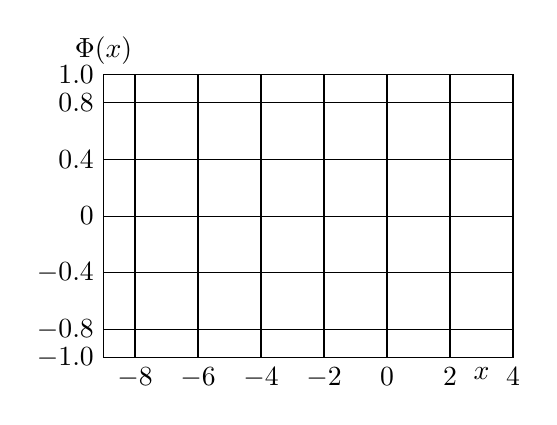
\begin{tikzpicture}[xscale=0.4,yscale=1.8]
	\draw (-9,-1)--(-9,1);
	\draw (-8,-1)--(-8,1);
	\draw (-6,-1)--(-6,1);
	\draw (-4,-1)--(-4,1);
	\draw (-2,-1)--(-2,1);
	\draw (0,-1)--(0,1);
	\draw (2,-1)--(2,1);
	\draw (4,-1)--(4,1);
	\draw (-9,-1)--(-9,1);
	\draw (-9,-1)--(4,-1);
	\draw (-9,-0.8)--(4,-0.8);
	\draw (-9,-0.4)--(4,-0.4);
	\draw (-9,0)--(4,0);
	\draw (-9,0.4)--(4,0.4);
	\draw (-9,0.8)--(4,0.8);
	\draw (-9,1)--(4,1);
	\draw plot[smooth] file{data};
	\node [below] at (-8,-1) {$ -8 $};
	\node [below] at (-6,-1) {$ -6 $};
	\node [below] at (-4,-1) {$ -4 $};
	\node [below] at (-2,-1) {$ -2 $};
	\node [below] at (0,-1) {$ 0 $};
	\node [below] at (2,-1) {$ 2 $};
	\node [below] at (4,-1) {$ 4 $};
	\node [left] at (-9,-1) {$ -1.0 $};
	\node [left] at (-9,-0.8) {$ -0.8 $};
	\node [left] at (-9,-0.4) {$ -0.4 $};
	\node [left] at (-9,0) {$ 0 $};
	\node [left] at (-9,0.4) {$ 0.4 $};
	\node [left] at (-9,0.8) {$ 0.8 $};
	\node [left] at (-9,1) {$ 1.0 $};
	\node [above] at (-9,1) {$ \Phi(x) $};
	\node [below] at (3,-1) {$ x $};
	\end{tikzpicture}\caption{FIG.55}\label{Fig.55}
\end{wrapfigure}
\begin{multline}\label{b.7}
\Phi'(x)=-\frac{x}{\sqrt{3\pi}}K_{2/3}\left(\frac{2}{3}x^{3/2} \right)\\
\text{ for }x>0.
\end{multline}


When $ x = 0 $,
\begin{equation}\label{b.8}
\begin{split}
\Phi(0)=\frac{\sqrt{\pi}}{3^{2/3}\Gamma(2/3)}=0.629,\\
\Phi'(0)=\frac{3^{1/6}\Gamma(2/3)}{2\sqrt{\pi}}=-0.459.
\end{split}
\end{equation}
Figure. \ref{Fig.55} shows a graph of the Airy function.



\section{Legendre polynomials\footnote{There are in the mathematical literature many good accounts of the theory of spherical harmonics. Here we shall give, for reference, only a few basic relations, and make no attempt at a systematic discussion of the theory of these functions.}}\label{Legendre polynomials}
The \textit{Legendre polynomials} $ P_l(\cos \theta) $ are defined by the formula
\begin{equation}\label{c.1}
P_l(\cos\theta)=\frac{1}{2^ll!}\frac{d^l}{(d\cos\theta)^l}(\cos^2\theta-1)^l.
\end{equation}



They satisfy the differential equation
\begin{equation}\label{c.2}
\frac{1}{\sin\theta}\frac{\d}{\d\theta}\left(\sin\theta\frac{\d P_l}{\d\theta} \right)+l(l+1)P_l=0.
\end{equation}
The associated Legendre polynomials are defined by
\begin{equation}\label{c.3}
P_l^m(\cos\theta)=\sin^m\theta\frac{\d^mP_l(\cos\theta)}{(\d\cos\theta)^m}=\frac{1}{2^ll!}\sin^m\theta\frac{\d^{l+m}}{(\d\cos\theta)^{l+m}}(\cos^2\theta-1)^l
\end{equation}
or, equivalently,
\begin{equation}\label{c.4}
P_l^m(\cos\theta)=(-1)^m\frac{(l+m)!}{(l-m)!2^ll!}\sin^{-m}\theta\frac{\d^{l-m}}{(\d\cos\theta)^{l-m}}(\cos^2\theta-1)^l,
\end{equation}
with $ m = 0, 1, \dots, l $. The associated polynomials satisfy the equation
\begin{equation}\label{c.5}
\frac{1}{\sin\theta}\frac{\d}{\d\theta}\left(\sin\theta\frac{\d P_l^m}{\d\theta} \right)+\left[l(l+1)-\frac{m^2}{\sin^2\theta} \right]P_l^m=0.
\end{equation}



The normalization integral $ \int_{-1}^{1}\left[P_l(\mu) \right]^2\d\mu (\mu=\cos \theta)$ for the Legendre polynomials is calculated by substituting \eqref{c.1} and integrating $ l $ times by parts, which gives
\[ \frac{(-1)^l}{2^{2l}(l!)^2}\int_{-1}^{1}(\mu^2-1)^l\frac{\d^{2l}}{{\d\mu}^{2l}}(\mu^2-1)^l\d\mu=\frac{(2l)!}{2^{2l}(l!)^2}\int_{-1}^{1}(1-\mu^2)^l\d\mu. \]
Substitution of $ u = (1 − \mu)/2 $ reduces this integral to Euler’s beta function, and the result is
\begin{equation}\label{c.6}
\int_{-1}^{1}[P_l(\mu)]^2\d\mu=\frac{2}{2l+1}.
\end{equation}
Similarly, it is easily seen that the functions $ P_l(\mu) $ with different $ l $ are orthogonal:
\begin{equation}\label{c.7}
\int_{-1}^{1}P_l(\mu)P_{l'}(\mu)\d\mu=0,l\ne l'.
\end{equation}



The calculation of the normalization integral for the associated Legendre polynomials is easily effected by a similar method. We write $ [P_l^m(\mu)]^2 $ as a product of the expressions \eqref{c.3} and \eqref{c.4}, and integrate $ l − m $ times by parts; the result is
\begin{equation}\label{c.8}
\int_{-1}^{1}[P_l^m(\mu)]^2\d\mu=\frac{2}{2l+1}\frac{(l+m)!}{(l-m)!}.
\end{equation}
It is also easily seen that the functions $ P_l^m $ with different $ l $ (and the same $ m $) are orthogonal:
\begin{equation}\label{c.9}
\int_{-1}^{1}P_l^m(\mu)P_{l'}^m(\mu)\d\mu=0,l\ne l'.
\end{equation}



The calculation of the integrals of products of three Legendre polynomials is discussed in \S107.

The following \textit{addition theorem} holds for Legendre polynomials. Let $\gamma$ be the angle between two directions defined by the spherical angles $ \theta, \phi $ and $ \theta', \phi': \cos \gamma = \cos \theta \cos \theta' + \sin \theta \sin \theta' \cos (\phi - \phi')$. Then
\begin{multline}\label{c.10}
P_l(\cos\gamma)=P_l(\cos\theta)P_l(\cos\theta')+\\
+\sum_{m-1}^{l}2\frac{(l-m)!}{(l+m)!}P_l^m(\cos\theta)P_l^m(\cos\theta')\cos[m(\phi-\phi')].
\end{multline}
This theorem can also be written in terms of the spherical harmonic functions defined by \eqref{28.7}:
\begin{equation}\label{c.11}
P_l(\bm{nn'})=\frac{4\pi}{2l+1}\sum_{m=-1}^l Y_{lm}^*(\bm{n'})Y_{lm}(\bm{n}).
\end{equation}



Here $ \bm{n} $ and $ \bm{n'} $ are two unit vectors, and $ Y_{lm}(\bm{n}) $ denotes the spherical harmonic function of the polar angle and azimuth of the direction of $ \bm{n} $ relative to a fixed system of coordinates.

If equation \eqref{c.10} is multiplied by $ P_{l'}(\cos \theta) $ and integrated over $ \d o = \sin \theta \d\theta \d\phi $, the integration with respect to $\phi$ gives zero for all terms on the right that contain factors $ \cos [m (\phi-  \phi')] $; using \eqref{c.6} and \eqref{c.7}, we obtain
\[ \int P_l(\cos\gamma)P_{l'}(\cos\theta)\d o=\delta_{ll'}\frac{4\pi}{2l+1}P_l(\cos\theta') .\]
This result may be written in the symmetrical form
\begin{equation}\label{c.12}
\int P_l(\bm{n}_1\bm{n}_2)P_{l'}(\bm{n_1}\bm{n_3})\d o_1=\delta_{ll'}\frac{4\pi}{2l+1}P_l(\bm{n}_2\bm{n}_3),
\end{equation}



where $ \bm{n}_1 , \bm{n}_2, \bm{n}_3$ are three unit vectors and the integration is with respect to the direction of $ \bm{n}_1 $.

Finally, we give the first few normalized spherical harmonics $ Y_{lm} $:
\[ Y_{00}=\frac{1}{\sqrt{4\pi}},\quad Y_{10}=\i\sqrt{\frac{3}{4\pi}}\cos\theta,\quad Y_{1,\pm1}=\pm\i\sqrt{\frac{3}{8\pi}}\sin\theta\cdot\e^{\pm\i\phi}, \]
\[ Y_{20}=\sqrt{\frac{5}{16\pi}}(1-3\cos^2\theta),\quad Y_{2,\pm1}=\pm\sqrt{\frac{15}{8\pi}}\cos\theta\sin\theta\cdot\e^{+\i\phi}, \]
\[ Y_{2,\pm2}=-\sqrt{\frac{15}{32\pi}}\sin^2\theta\cdot\e^{\pm2\i\phi},\quad Y_{30}=-\i\sqrt{\frac{7}{16\pi}}\cos\theta(5\cos^2\theta-3), \]
\[ Y_{3,\pm1}=\pm\i\sqrt{\frac{21}{64\pi}}\sin\theta(5\cos^2\theta-1)\e^{\pm\i\phi}, \]
\[ Y_{3,\pm2}=-\i\sqrt{\frac{105}{32\pi}}\cos\theta\sin^2\theta\cdot\e^{\pm2\i\phi},\quad Y_{3,\pm3}=\pm\i\sqrt{\frac{35}{64\pi}}\sin^3\theta\cdot\e^{\pm3\i\phi}. \]
\section{The confluent hypergeometric function}\label{The confluent hypergeometric function}
The \textit{confluent hypergeometric function} is defined by the series
\begin{equation}\label{d.1}
F(\alpha,\gamma,z)=1+\frac{\alpha}{\gamma}\frac{z}{1!}+\frac{\alpha(\alpha+1)}{\gamma(\gamma+1)}\frac{z^2}{2!}+\dots,
\end{equation}
which converges for all finite $ z $; the parameter $\alpha$ is arbitrary, while the parameter $\gamma$ is supposed not zero or a negative integer. If $\alpha$ is a negative integer (or zero), $ F (\alpha, \gamma, z) $ reduces to a polynomial of degree $ |\alpha| $.

The function $ F (\alpha, \gamma, z) $ satisfies the differential equation
\begin{equation}\label{d.2}
zu''+(\gamma-z)u'-\alpha u=0,
\end{equation}
as is easily seen by direct verification.\footnote{The equation \eqref{d.2} with a negative integral $\gamma$ does not require special discussion, since it can be reduced to a case of positive integral $\gamma$ by the transformation which gives equation \eqref{d.3}.
} By the substitution $ u = z^{1-\gamma} u_1 $, this equation is transformed into another of the same form,
\begin{equation}\label{d.3}
zu_1''+(2-\gamma-z)u_1'-(\alpha-\gamma+1)u_1=0.
\end{equation}
Hence we see that, for non-integral $\gamma$, equation \eqref{d.2} has also the particular integral $ z^{1-\gamma}F (\alpha-\gamma+1, 2-\gamma, z) $, which is linearly independent of \eqref{d.1}, so that the general solution of equation \eqref{d.2} is of the form
\begin{equation}\label{d.4}
u=c_1F(\alpha,\gamma,z)+c_2z^{1-\gamma}F(\alpha-\gamma+1,2-\gamma,z).
\end{equation}
The second term, unlike the first, has a singular point at $ z = 0 $.

Equation \eqref{d.2} is of Laplace’s type, and its solutions can be represented as contour integrals. Following the general method, we form the functions
\[ P(t)=\gamma t-\alpha,\quad Q(t)=t(t-1),\quad Z(t)=t^{\alpha-1}(t-1)^{\gamma-\alpha-1}, \]
so that
\begin{equation}\label{d.5}
u=\int\e^{tz}t^{\alpha-1}(t-1)^{\gamma-\alpha-1}\d t.
\end{equation}
The path of integration must be chosen so that the function $ V(t) = \e^{tz}t^\alpha (t - 1)^{\gamma-\alpha} $ returns to its original value on traversing the path. Applying the same method to equation \eqref{d.3}, we can obtain for u a contour integral of another form:
\[ u=z^{1-\gamma}\int\e^{tz}t^{\alpha-\gamma}(t-1)^{-\alpha}\d t. \]
The substitution $ tz \to t $ reduces this integral to the convenient form
\begin{equation}\label{d.6}
u(z)=\int\e^t(t-z)^{-\alpha}t^{\alpha-\gamma}\d t,
\end{equation}
and the corresponding function $ V $ to
\[ V(t)=\e^t(t-z)^{-\alpha}t^{\alpha-\gamma}\d t, \]



The integrand in \eqref{d.6} has in general two singular points, at $ t = z $ and $ t = 0 $. We take a contour of integration $ C $ which passes from infinity ($ \text{Re}t \to-\infty $)
\begin{wrapfigure}[]{l}[0cm]{0cm}
	\begin{tikzpicture}[scale=0.7]
	\draw (-6,-2)[-{Stealth[length=3pt, angle'=60]}]--(-3,-2);
	\draw (-4,-2)--(0,-2);
	\draw (0,-2)[-{Stealth[length=3pt, angle'=60]}]--(0,-2)arc[radius = 2cm, start angle = -90, delta angle = 90];
	\draw (2,0)--(2,0)arc[radius = 2cm, start angle = 0, delta angle = 90];
	\draw (0,2)[-{Stealth[length=3pt, angle'=60]}]--(-3,2);
	\draw (-2,2)--(-6,2);
	
	\draw (-6,-1.5)[-{Stealth[length=3pt, angle'=60]}]--(-3,-1.5);
	\draw (-4,-1.5)--(0,-1.5);
	\draw (0,-1.5)arc[radius = 0.25cm, start angle = -90, delta angle = 180];
	\draw (0,-1)[-{Stealth[length=3pt, angle'=60]}]--(-3,-1);
	\draw (-2,-1)--(-6,-1);
	
	\draw (-6,1)[-{Stealth[length=3pt, angle'=60]}]--(-3,1);
	\draw (-4,1)--(0,1);
	\draw (0,1)arc[radius = 0.25cm, start angle = -90, delta angle = 180];
	\draw (0,1.5)[-{Stealth[length=3pt, angle'=60]}]--(-3,1.5);
	\draw (-2,1.5)--(-6,1.5);
	\fill (0,-1.25) circle(1.5pt);
	\node [left,font=\scriptsize] at (0,-1.25) {$ t=0 $};
	\fill (0,1.25) circle(1.5pt);
	\node [left,font=\scriptsize] at (0,1.25) {$ t=Z $};
	\draw[dashed] (0,1.25)--(0,-1.25);
	\node[right,font=\scriptsize] at (0.25,-1.25) {$ C_1 $};
	\node[right,font=\scriptsize] at (0.25,1.25) {$ C_2 $};
	\node[right,font=\scriptsize] at (2,0) {$ C $};
	\end{tikzpicture}\caption{FIG. 56}\label{Fig.56}
\end{wrapfigure}
round the two singular points in the positive direction and back to infinity (Fig. \ref{Fig.56}). This contour satisfies the required conditions, since $ V (t) $ vanishes at its ends. The integral \eqref{d.6}, taken along the contour $ C $, has no singular point for $ z = 0 $; hence it must be the same, apart from a constant factor, as the function $ F (\alpha, \gamma, z) $, which also has no singularity. For $ z = 0 $ the two singular points of the integrand coincide; according to a well-known formula in the theory of the gamma function,
\begin{equation}\label{d.7}
\frac{1}{2\pi\i}\int_C\e^tt^{-\gamma}\d t=\frac{1}{\Gamma(\gamma)}.
\end{equation}
Since $ F (\alpha, \gamma, 0)=1 $, it is evident that
\begin{equation}\label{d.8}
F (\alpha, \gamma, z) =\frac{\Gamma(\gamma)}{2\pi\i}\int_C\e^t(t-z)^{-\alpha}t^{\alpha-\gamma}\d t.
\end{equation}
The integrand in \eqref{d.5} has singular points at $ t = 0 $ and $ t = 1 $.
\begin{wrapfigure}[6]{r}[0cm]{0cm}
	\begin{tikzpicture}[xscale=1.75,yscale=0.875]
	\draw [-{Stealth[length=3pt, angle'=60]}][domain=-45:-28,scale=1.5,samples=500] plot (\x:{-(2* cos(2*\x))^0.5});
	\draw [-{Stealth[length=3pt, angle'=60]}][domain=-30:28,scale=1.5,samples=500] plot (\x:{-(2* cos(2*\x))^0.5});
	\draw [domain=0:45,scale=1.5,samples=500] plot (\x:{-(2* cos(2*\x))^0.5});
	\draw[-] (-2.5,0)--(0.5,0);
	\fill[xscale=0.5] (-3.5,0) circle(1.5pt);
	\node[font=\scriptsize,above] at (-1.8,0) {$ t=0 $}; 
	\fill[xscale=0.5] (0,0) circle(1.5pt);
	\node[font=\scriptsize,below] at (0,0) {$ t=1 $}; 
	\node[font=\scriptsize] at (-2,-1) {$ C' $}; 
	\end{tikzpicture}\caption{FIG. 57}\label{Fig.57}
\end{wrapfigure} 
If $ \mathrm{Re}(\gamma-\alpha) > 0 $,
and $\gamma$ is not a positive integer, the path of integration can be taken as a contour $ C' $ starting from the point $ t = 1 $, passing round the point $ t = 0 $ in the positive direction, and returning to $ t = 1 $ (Fig. \ref{Fig.57}); for $ \mathrm{Re}(\gamma-\alpha) > 0 $, the function $ V (t) $ returns to its original value of zero on passing round such a contour.\footnote{If $\gamma$ is a positive integer, $ C' $ can be any contour which passes round both the points $ t = 0 $ and $ t = 1 $} The integral thus defined again has no singularity for $ z = 0 $, and is related to $ F (\alpha, \gamma, z) $ by
\begin{equation}\label{d.9}
F(\alpha, \gamma, z)=-\frac{1}{2\pi\i}\frac{\Gamma(1-\alpha)\Gamma(\gamma)}{\Gamma(\gamma-\alpha)}\oint_{C'}\e^{tz}(-t)^{\alpha-1}(1-t)^{\gamma-\alpha-1}\d t.
\end{equation}





The following remark should be made concerning the integrals \eqref{d.8}, \eqref{d.9}. For non-integral $\alpha$ and $\gamma$, the integrands are not one-valued functions. Their values at each point are supposed chosen in accordance with the condition that the complex quantity which is raised to a power is taken with the argument whose absolute value is least.

We may notice the useful relation
\begin{equation}\label{d.10}
F(\alpha,\gamma,z)=\e^zF(\gamma-\alpha,\gamma,-z),
\end{equation}
which is obtained at once by substituting $ t \to t + z $ in the integral \eqref{d.8}.

We have already remarked that, if $ \alpha = -n $, where $ n $ is a positive integer, the function $ F (\alpha, \gamma, z) $ reduces to a polynomial. A concise formula can be obtained for these polynomials. Making in the integral \eqref{d.9} the substitution $ t \to 1-(t/z) $ and applying Cauchy’s formula to the resulting integral, we find
\begin{equation}\label{d.11}
F(-n,\gamma,z)=\frac{1}{\gamma(\gamma+1)\dots(\gamma+n-1)}z^{1-\gamma}\e^z\frac{\d^m}{{\d z}^n}(\e^{-z}z^{\gamma+n-1}).
\end{equation}
If also $ \gamma = $ a positive integer $ m $, we have the formula
\begin{equation}\label{d.12}
F(-n,m,z)=\frac{(-1)^{m-1}}{m(m+1)\dots(m+n-1)}\e^z\frac{\d^{m+n-1}}{{\d z}^{m+n-1}}(\e^{-z}z^n).
\end{equation}
This formula is obtained by applying Cauchy’s formula to the integral derived from \eqref{d.8} by the substitution $ t \to z - t $.

The polynomials $ F (-n, m, z), 0 \leqslant m \leqslant n $, are (apart from a constant factor) the \textit{generalized Laguerre polynomials}
\begin{multline}\label{d.13}
L_n^m(z)=(-1)^m\frac{(n!)^2}{m!(n-m)!}F(-(n-m),m+1,z)=\\
=\frac{n!}{(n-m)!}\e^z\frac{\d^n}{{\d z}^n}\e^{-z}z^{n-m}=(-1)^m\frac{n!}{(n-m)!}\e^zz^{-m}\frac{\d^{n-m}}{{\d z}^{n-m}}\e^{-z}z^n.
\end{multline}
The polynomials $ L_n^m $ for $ m = 0 $ are denoted by $ L_n(z) $ and are called simply \textit{Laguerre polynomials}; from \eqref{d.13} we have
\[ L_n)z =\e^z\frac{\d^n}{{\d z}^n}(\e^{-z}z^n). \]



The integral representation \eqref{d.8} is convenient for obtaining the asymptotic expansion of the confluent hypergeometric function for large $ z $. We deform the contour into two contours $ C_1 $ and $ C_2 $ (Fig. 56), which pass round the points $ t = 0 $ and $ t = z $ respectively; the lower branch of $ C_2 $ and the upper branch of $ C_1 $ are supposed to join at infinity. To obtain an expansion in inverse powers of $ z $, we take $ (-z)^{-\alpha} $ outside the parenthesis in the integrand. In the integral along the contour $ C_2 $, we make the substitution $ t \to t + z $; the contour $ C_2 $ is thereby transformed into $ C_1 $ We thus represent the formula \eqref{d.8} as
\begin{multline}\label{d.14}
F(\alpha,\gamma,z)=\frac{\Gamma(\gamma)}{\Gamma(\gamma-\alpha)}(-z)^{-\alpha}G(\alpha,\alpha-\gamma+1,-z)+\\
+\frac{\Gamma(\gamma)}{\Gamma(\alpha)}\e^z z^{\alpha-\gamma}G(\gamma-\alpha,1-\alpha,z),
\end{multline}
where
\begin{equation}\label{d.15}
G(\alpha,\beta,z)=\frac{\Gamma(1-\beta)}{2\pi\i}\int_{C_1}\left(1+\frac{t}{z} \right)^{-\alpha}t^{\beta-1}\e^t\d t.
\end{equation}
In raising $ -z $ and $ z $ to powers in the formula \eqref{d.14} we must take the arguments which have the smallest absolute value. Finally, expanding $ (1 + t/z)^{-\alpha} $ in the integrand in powers of $ t/z $ and applying formula \eqref{d.7}, we have for $ G (\alpha, \beta, z) $ the asymptotic series
\begin{equation}\label{d.16}
G(\alpha,\beta,z)=1+\frac{\alpha\beta}{1!z}+\frac{\alpha(\alpha+1)\beta(\beta+1)}{2!z^2}+\dots
\end{equation}
Formulae \eqref{d.14} and \eqref{d.16} give the asymptotic expansion of the function $ F (\alpha, \gamma, z) $.

For positive integral $\gamma$, the second term in the general solution \eqref{d.4} of equation \eqref{d.2} is either the same as the first term (if $ \gamma = 1 $) or meaningless (if $ \gamma > 1 $). In this case we can take, as a set of two linearly independent solutions, the two terms in formula \eqref{d.14}, i.e. the integrals \eqref{d.8} taken along the contours $ C_1 $ and $ C_2 $ (these contours, like $ C $, satisfy the required conditions, so that the integrals along them are solutions of equation \eqref{d.2}). The asymptotic form of these solutions is given by the formulae already obtained; it remains for us to find their expansion in ascending powers of $ z $. To do this, we start from equation \eqref{d.14} and the analogous equation for the function $ z^{1-\gamma} F (\alpha-\gamma + 1, 2 -\gamma, z) $. From these two equations we express $ G (\alpha, \alpha-\gamma  + 1, - z) $ in terms of $ F (\alpha, \gamma, z) $ and $ F (\alpha-\gamma  + 1, 2 -\gamma, z) $; we then put $ \gamma= p + \epsilon  $($ p $ being a positive integer), and pass to the limit $ \epsilon\to0 $, resolving the indeterminacy by L’Hospital’s rule. A fairly lengthy calculation gives the following expansion:
\begin{multline}\label{d.17}
G(\alpha,\alpha-p+1,-z)=\frac{\sin\pi\alpha\cdot\Gamma(p-a)}{\pi\Gamma(p)}z^\alpha\times\\
\times\left\{\ln z\cdot F(\alpha,p,z)
+\sum_{s=0}^\infty\frac{\Gamma(p)\Gamma(\alpha+s)\left[\psi(\alpha+s)-\psi(p+s)-\psi(s+1) \right]}{\Gamma(\alpha)\Gamma(s+p)\Gamma(s+1)}z^s+\right.\\
\left.+\sum_{s=1}^{p-1}(-1)^{s+1}\frac{\Gamma(s)\Gamma(\alpha-s)\Gamma(p)}{\Gamma(\alpha)\Gamma(p-s)}z^{-s}    \right\},
\end{multline}
where $\psi$ denotes the logarithmic derivative of the gamma function: $ \psi(\alpha = \Gamma'(\alpha)/\Gamma(\alpha) $.
\section{The hypergeometric function}\label{The hypergeometric function}
The \textit{hypergeometric function} is defined in the circle $ |z| < 1 $ by the series
\begin{equation}\label{e.1}
F(\alpha,\beta,\gamma,z)=1+\frac{\alpha\beta}{\gamma}\frac{z}{1!}+\frac{\alpha(\alpha+1)\beta(\beta+1)}{\gamma(\gamma+1)}\frac{z^2}{2!}+\dots,
\end{equation}
and for $ |z| > 1 $ it is obtained by analytical continuation of this series (see \eqref{e.6}). The hypergeometric function is a particular integral of the differential equation
\begin{equation}\label{e.2}
z(1-z)u''+[\gamma-(\alpha+\beta+1)z]u'-\alpha\beta u=0.
\end{equation}
The parameters $\alpha$ and $\beta$ are arbitrary, while $ γ \ne 0, -1, -2, \dots $ The function $ F (\alpha, \beta, \gamma, z) $ is evidently symmetrical with respect to the parameters $\alpha$ and $\beta$.\footnote{The confluent hypergeometric function is obtained from $ F (\alpha, \beta, \gamma, z) $ by taking the limit
\[ F (\alpha, \gamma, z)=\lim\limits_{\beta\to\infty}F (\alpha, \beta, \gamma, \frac{z}{\beta}) \]
	
	
	
The notation$ {}_2F_1(\alpha, \beta, \gamma, z) $ for the hypergeometric function and $ {}_1F_1(\alpha, \gamma, z) $ for the confluent hypergeometric function is also used in the literature. The subscripts to the left and right of $ F $ show the numbers of parameters in the numerators and denominators respectively of the terms in the series.
} The second independent solution of equation \eqref{e.2} is
\[ z^{1-\gamma}F(\beta-\gamma+1,\alpha-\gamma+1,2-\gamma,z); \]
it has a singular point at $ z = 0 $.

We shall give here for reference a number of relations obeyed by the hypergeometric function.

The function $ F (\alpha, \beta, \gamma, z) $ can be represented for all $ z $, if $ \mathrm{Re}(γ − α) > 0 $, as an integral:
\begin{multline}\label{e.3}
F(\alpha,\beta,\gamma,z)=\\
=-\frac{1}{2\pi\i}\frac{\Gamma(1-\alpha)\Gamma(\gamma)}{\Gamma(\gamma-\alpha)}\oint_{C'}(-t)^{\alpha-1}(1-t)^{\gamma-\alpha-1}(1-tz)^{-\beta}\d t,
\end{multline}
taken along the contour $ C' $ shown in Fig. \ref{Fig.57}. That this integral in fact satisfies equation \eqref{e.2} is easily seen by direct substitution; the constant factor is chosen so as to give unity for $ z = 0 $.

The substitution $ u = (1 - z)^{\gamma-\alpha-\beta}u_1 $ in equation \eqref{e.2} leads to an equation of the same form, with parameters $ \gamma-\alpha, \gamma-\beta, \gamma $ in place of $ \alpha, \beta, \gamma $ respectively. Hence we have
\begin{equation}\label{e.4}
F(\alpha,\beta,\gamma,z)=(1-z)^{\gamma-\alpha-\beta}F(\gamma-\alpha,\gamma-\beta,\gamma,z)
\end{equation}
both sides of this equation satisfy the same equation, and they have the same value for $ z = 0 $.

The substitution $ t \to t/(1 - z + zt) $ in the integral \eqref{e.3} leads to the following relation between hypergeometric functions with variables $ z $ and $ z/(z − 1) $:
\begin{equation}\label{e.5}
F(\alpha,\beta,\gamma,z)=(1-z)^{-\alpha}F\left(\alpha,\gamma-\beta,\gamma,\frac{z}{z-1}\right).
\end{equation}
The value of the many-valued expression $ (1 - z)^{-\alpha} $ in this formula (and of similar expressions in all the following formulae) is determined by the condition that the complex quantity which is raised to a power is taken with the argument whose absolute value is least.

Next we shall give, without proof, an important formula relating hypergeometric functions with variables $ z $ and $ 1/z $:
\begin{multline}\label{e.6}
F(\alpha,\beta,\gamma,z)=\frac{\Gamma(\gamma)\Gamma(\beta-\alpha)}{\Gamma(\beta)\Gamma(\gamma-\alpha)}(-z)^{-\alpha}F\left(\alpha,\alpha+1-\gamma,\alpha+1-\beta,\frac{1}{z}\right)+\\
+\frac{\Gamma(\gamma)\Gamma(\alpha-\beta)}{\Gamma(\alpha)\Gamma(\gamma-\beta)}(-z)^{-\beta}F\left(\beta,\beta+1-\gamma,\beta+1-\alpha,\frac{1}{z} \right).
\end{multline}
This formula expresses $ F (\alpha, \beta, \gamma, z) $ as a series which converges for $ |z| > 1 $, i.e. it is the analytical continuation of the original series \eqref{e.1}.

The formula
\begin{multline}\label{e.7}
F(\alpha,\beta,\gamma,z)=\frac{\Gamma(\gamma)\Gamma(\gamma-\alpha-\beta)}{\Gamma(\gamma-\alpha)\Gamma(\gamma-\beta)}F(\alpha,\beta,\alpha+\beta+1-\gamma,1-z)+\\
+\frac{\Gamma(\gamma)\Gamma(\alpha+\beta-\gamma)}{\Gamma(\alpha)\Gamma(\beta)}(1-z)^{\gamma-\alpha-\beta}F(\gamma-\alpha,\gamma-\beta,\gamma+1-\alpha-\beta,1-z).
\end{multline}
relates hypergeometric functions of $ z $ and $ 1 - z $; again, the proof will not be given here. Combining \eqref{e.7} with \eqref{e.6}, we obtain the relations
\begin{multline}\label{e.8}
F(\alpha,\beta,\gamma,z)=\frac{\Gamma(\gamma)\Gamma(\beta-\alpha)}{\Gamma(\beta)\Gamma(\gamma-\alpha)}(1-z)^{-\alpha}F\left(\alpha,\gamma-\beta,\alpha+1-\beta,\frac{1}{1-z} \right)+\\
+\frac{\Gamma(\gamma)\Gamma(\alpha-\beta)}{\Gamma(\alpha)\Gamma(\gamma-\beta)}(1-z)^{-\beta}F(\beta,\gamma-\alpha,\beta+1-\alpha,\frac{1}{1-z}),
\end{multline}
\begin{multline}\label{e.9}
F(\alpha,\beta,\gamma,z)=\frac{\Gamma(\gamma)\Gamma(\gamma-\alpha-\beta)}{\Gamma(\gamma-\beta)\Gamma(\gamma-\alpha)}\times\\
\times z^{-\alpha}F\left(\alpha,\alpha+1-\gamma,\alpha+\beta+1-\gamma,\frac{z-1}{z} \right)+\frac{\Gamma(\gamma)\Gamma(\alpha+\beta-\gamma)}{\Gamma(\alpha)\Gamma(\beta)}\times\\
\times(1-z)^{\gamma-\alpha-\beta}z^{\beta-\gamma}F\left(1-\beta,\gamma-\beta,\gamma+1-\alpha-\beta,\frac{z-1}{z} \right).
\end{multline}
Each of the terms in the sums on the right of equations \eqref{e.6}--\eqref{e.9} is itself a solution of the hypergeometric equation.

If $\alpha$ (or $\beta$) is a negative integer or zero, $ \alpha = -n $, the hypergeometric function reduces to a polynomial of the $ n $th degree, and can be represented in the form
\begin{equation}\label{e.10}
F(-n,\beta,\gamma,z)=\frac{z^{1-\gamma}(1-z)^{\gamma+n-\beta}}{\gamma(\gamma+1)\dots(\gamma+n-1)}\frac{\d^n}{{\d z}^n}\left[z^{\gamma+n-1}(1-z)^{\beta-\gamma} \right].
\end{equation}
These polynomials are the same, apart from a constant factor, as the \textit{Jacobi polynomials}, defined by
\begin{multline}\label{e.11}
P_n^{(a,b)}(z)=\frac{(a+1)(a+2)\dots(a+n)}{n!}F\left(-n,a+b+n+1,a+1,\frac{1-z}{2} \right)=\\
=\frac{(-1)^n}{2^n n!}(1-z)^{-a}(1+z)^{-b}\frac{\d^n}{{\d z}^n}\left[(1-z)^{a+n}(1+z)^{b+n} \right].
\end{multline}
For $ a = b = 0 $, the Jacobi polynomials are the Legendre polynomials. For $ n = 0 $, $ P_0^{(a, b)} = 1 $.




\section{The calculation of integrals containing confluent hypergeometric functions}\label{The calculation of integrals containing confluent hypergeometric functions}
Let us consider an integral of the form
\begin{equation}\label{f.1}
J_{\alpha\gamma}^\nu=\int_{0}^{\infty}\e^{-\lambda z}z^\nu F(\alpha,\gamma,kz)\d z.
\end{equation}
We assume that it converges. If this is so we must have $ \mathrm{Re} \nu > -1 $ and $ \mathrm{Re}\lambda >| \mathrm{Re} k| $; if $\alpha$ is a negative integer, the latter condition can be replaced by $ \mathrm{Re}\lambda >0$. Using for $ F (\alpha, \gamma, kz) $ the integral representation \eqref{d.9} and effecting the integration over $ z $ under the contour integral, we have
\begin{multline*}
J_{\alpha\gamma}^\nu=-\frac{1}{2\pi\i}\frac{\Gamma(1-\alpha)\Gamma(\gamma)}{\Gamma(\gamma-\alpha)}\lambda^{-\nu-1}\Gamma(\nu+1)\times\\
\times\oint_{C'}(-t)^{\alpha-1}(1-t)^{\gamma-\alpha-1}(1-(k/\lambda)t)^{-\nu-1}\d t.
\end{multline*}



Using \eqref{e.3}, we have finally
\begin{equation}\label{f.2}
J_{\alpha\gamma}^\nu=\Gamma(\nu+1)\lambda^{-\nu-1}F(\alpha,\nu+1,\gamma,k/\lambda).
\end{equation}
In the cases where the function $ F (\alpha, \nu + 1, \gamma, k/\lambda) $ reduces to a polynomial, we have for the integral $ J_{\alpha\gamma}^\nu $ an expression in terms of elementary functions:
\begin{equation}\label{f.3}
J_{\alpha\gamma}^{\gamma+n-1}=(-1)^n\Gamma(\gamma)\frac{\d^n}{{\d\lambda}^n}\left[\lambda^{\alpha-\gamma}(\lambda-k)^{-\alpha} \right],
\end{equation}
\begin{equation}\label{f.4}
J_{-n\gamma}^\nu=(-1)^n\frac{\Gamma(\nu+1)(\lambda+k)^{\gamma+n-\nu-1}}{\gamma(\gamma+1)\dots(\gamma+n-1)}\frac{\d^n}{{\d\lambda}^n}\left[\lambda^{-\nu-1}(\lambda-k)^{\nu-\gamma+1} \right],
\end{equation}
\begin{multline}\label{f.5}
J_{\alpha m}^n=\frac{(-1)^{m-n}}{k^{m-1}(1-\alpha)(2-\alpha)\dots(m-1-\alpha)}\times\\
\times\left\{-(m-1)!\frac{\d^n}{{\d\lambda}^n}\left[\lambda^{\alpha-1}(\lambda-k)^{m-\alpha-1} \right]+\right.\\
+n!(m-n-1)\dots(m-1)\lambda^{\alpha-n-1}(\lambda-k)^{-1+m-n-\alpha}\times\\
\times\left.\frac{\d^{m-n-2}}{{\d\lambda}^{m-n-2}}\left[\lambda^{m-\alpha-1}(\lambda-k)^{\alpha-1} \right]\right\};
\end{multline}
here $ m, n $ are integers, with $ 0 \leqslant n \leqslant m - 2 $.

Next, let us calculate the integral
\begin{equation}\label{f.6}
J_\nu=\int_{0}^{\infty}\e^{-kz}z^{\nu-1}\left[F(-n,\gamma,kz) \right]^2\d z,
\end{equation}
where $ n $ is an integer and $ \text{Re } v > 0 $. To calculate this, we begin with a more general integral having $ \e^{-\lambda z} $ instead of $ \e^{-ks} $ in the integrand. We write one of the functions $ F (-n, \gamma, kz) $ as a contour integral \eqref{d.9}, and then integrate over $ z $, using formula \eqref{f.3}:
\begin{multline*}
\int_{0}^{\infty}=\e^{-\lambda z}z^{\nu-1}\left[F(-n,\gamma,kz) \right]^2\d z=-\frac{1}{2\pi\i}(-1)^n\frac{\Gamma(1+n)\Gamma^2(\gamma)\Gamma(\nu)}{\Gamma^2(\gamma+n)}\times\\
\times\oint_{C'}(\lambda-kt-k)^{\gamma+n-\nu}(-t)^{-n-1}(1-t)^{\gamma+n-1}\times\\
\times\frac{\d^n}{{\d\lambda}^n}\left[(\lambda-kt)^{-\nu}(\lambda-kt-k)^{\nu-\gamma} \right]\d t.
\end{multline*}
The $ n $th derivative with respect to $\lambda$ can evidently be replaced by a derivative of the same order with respect to $ t $; we then put $ \lambda = k $, and thereby return to the integral $ J_\nu $:
\begin{multline*}
J_\nu=-\frac{1}{2\pi\i}\frac{\Gamma(n+1)\Gamma(\nu)\Gamma^2(\gamma)}{\Gamma^2(\gamma+n)k^\nu}\times\\
\times\oint_{C'}(-t)^{\gamma-\nu-1}(1-t)^{\gamma+n-1}\frac{\d^n}{{\d t}^n}\left[(1-t)^{-\nu}(-t)^{\nu-\gamma} \right]\d t.
\end{multline*}
By integrating $ n $ times by parts, we transfer the operator $ \d^n/{\d t}^n $ to the expression $ (-t)^{\gamma-\nu-1} (1 - t)^{\gamma+n-1} $, and then expand the derivative by Leibniz’ formula. As a result, we obtain a sum of integrals, each of which reduces to Euler’s well-known integral. We finally have the following expression for the integral required:
\begin{multline}\label{f.7}
J_\nu=\frac{\Gamma(\nu)n!}{k^\nu\gamma(\gamma+1)\dots(\gamma+n-1)}\times\\
\times\left\{1+\sum_{s=0}^{n-1}\frac{n(n-1)\dots(n-s)(\gamma-\nu-s-1)(\gamma-\nu-s)\dots(\gamma-\nu+s)}{[(s+1)!]^2\gamma(\gamma+1)\dots(\gamma+s)}
 \right\}.
\end{multline}
It is easy to see that the integrals $ J_\nu $ are related by
\begin{equation}\label{f.8}
J_{\gamma+p}=\frac{(\gamma-p-1)(\gamma-p)\dots(\gamma+p-1)}{k^{2p+1}}J_{\gamma-1-p},
\end{equation}
where $ p $ is any integer.

We similarly calculate the integral
\begin{equation}\label{f.9}
J=\int_{0}^{\infty}\e^{-\lambda z}z^{\gamma-1}F(\alpha,\gamma,kz)F(\alpha',\gamma,k'z)\d z.
\end{equation}
We represent the function $ F (\alpha', \gamma, k'z) $ as a contour integral \eqref{d.9}, and integrate over $ z $, using formula \eqref{f.3} with $ n = 0 $:
\begin{multline*}
J=-\frac{1}{2\pi\i}\frac{\Gamma(1-\alpha')\Gamma^2(\gamma)}{\Gamma(\gamma-\alpha')}\oint_{C'}(-t)^{\alpha'-1}(1-t)^{\gamma-\alpha'-1}(\lambda-k't)^{\alpha-\gamma}\times\\
\times(\lambda-k't-k)^{-\alpha}\d t.
\end{multline*}



By the substitution $ t \to \lambda t/(k't + \lambda - k') $, this integral is brought to the form \eqref{e.3}, giving
\begin{equation}\label{f.10}
J=\Gamma(\gamma)\lambda^{\alpha+\alpha'-\gamma}(\lambda-k)^{-\alpha}(\lambda-k')^{-\alpha'}F\left(\alpha,\alpha',\gamma,\frac{kk'}{(\lambda-k)(\lambda-k')} \right).
\end{equation}
If $\alpha$ (or $ \alpha' $) is a negative integer, $ \alpha = -n $, this expression can be rewritten, using \eqref{e.7}, as
\begin{multline}\label{f.11}
J=\frac{\Gamma^2(\gamma)\Gamma(\gamma+n-\alpha')}{\Gamma(\gamma+n)\Gamma(\gamma-\alpha')}\lambda^{-n+\alpha'-\gamma}(\lambda-k)^n(\lambda-k')^{-\alpha'}\times\\
\times F(-n,\alpha',-n+\alpha'+1-\gamma,\frac{\lambda(\lambda-k-k')}{(\lambda-k)(\lambda-k')}).
\end{multline}



Finally, let us consider integrals of the form
\begin{equation}\label{f.12}
J_\nu^{sp}(\alpha,\alpha')=\int_{0}^{\infty}\exp\left(-\frac{k+k'}{2}z \right)z^{\gamma-1+s}F(\alpha,\gamma,kz)F(\alpha',\gamma-p,k'z)\d z.
\end{equation}
The values of the parameters are supposed such that the integral converges absolutely; $ s $ and $ p $ are positive integers. The simplest of these integrals, $ J_\gamma^{00}(\alpha,\alpha') $, is by \eqref{f.10},
\begin{multline}\label{f.13}
J_\nu^{00}(\alpha,\alpha')=2^\gamma\Gamma(\gamma)(k+k')^{\alpha+\alpha'-\gamma}(k'-k)^{-\alpha}\times\\
\times(k-k')^{-\alpha'}F\left(\alpha,\alpha',\gamma,-\frac{4kk'}{(k'-k)^2} \right),
\end{multline}
if $\alpha$ (or $\alpha'$) is a negative integer, $ \alpha = -n $, we can also write, by \eqref{f.11},
\begin{multline}\label{f.14}
J_\gamma^{00}(-n,\alpha')=2^\gamma\frac{\Gamma(\gamma)(\gamma-\alpha')(\gamma-\alpha'+1)\dots(\gamma-\alpha'+n-1)}{\gamma(\gamma+1)\dots(\gamma+n-1)}\times\\
\times(-1)^n(k+k')^{-n+\alpha'-\gamma}(k-k')^{n-\alpha'}\times\\
\times F\left[-n,\alpha',\alpha'+1-n-\gamma,\left(\frac{k+k'}{k-k'} \right)^2\right].
\end{multline}
The general formula for $ J_\gamma^{sp}(\alpha, \alpha') $ can be derived, but it is so complex that it cannot be used conveniently. It is more convenient to use recurrence formulae, which enable us to reduce the integrals $ J_\gamma^{sp}(\alpha, \alpha') $ to the integral with $ s = p = 0 $. The formula
\begin{equation}\label{f.15}
J_\gamma^{sp}(\alpha,\alpha')=\frac{\gamma-1}{k}\{J_{\gamma-1}^{s,p-1}(\alpha,\alpha')-J_{\gamma-1}^{s,p-1}(\alpha-1,\alpha') \}
\end{equation}
enables us to reduce $ J_\gamma^{sp}(\alpha,\alpha') $ to the integral with $ p = 0 $. The formula
\begin{multline}\label{f.16}
J_\gamma^{s+1,0}(\alpha,\alpha')=\frac{4}{k^2-{k'}^2}\{[\gamma(k-k')/2-k\alpha+k'\alpha-k's]J_\gamma^{s0}(\alpha,\alpha')+\\
+s(\gamma-1+s-2\alpha')J_\gamma^{s-1,0}(\alpha,\alpha')+2\alpha' sJ_\gamma^{s-1,0}(\alpha,\alpha+1)\}
\end{multline}
then makes possible the final reduction to the integral with $ s = p = 0 $.\footnote{See W. Gordon, \textit{Annalen der Physik} [5] 2, 1031, 1929.}



